\section{Method}
This section aims to describe the technologies we intend to use, and how we intend to use them, to solve the tasks described in the problem section.

The subproblems in section \ref{sec:problem} have been divided further into the generators found in figure \ref{fig:generators}. 
The basic notion is that these generators will be called from a root level in code and that the result of one or more generators will be feed into the next generator.
Figure~\ref{fig:generatorexamples} shows three of the different generators and how they can be visualized on a 2D plane. 

\begin{center}
  \begin{figure}[H]
    \begin{center}
      \begin{table}[H]
        \begin{tabular}{lllll}
          \textit{User parameters}              & $\rightarrow$ & \textbf{TerrainGenerator}    & $\rightarrow$ & \textit{Terrain}        \\
          \textit{Terrain, Population markers}  & $\rightarrow$ & \textbf{PopulationGenerator} & $\rightarrow$ & \textit{Population map} \\
          \textit{Terrain, Population map}      & $\rightarrow$ & \textbf{RoadGenerator}       & $\rightarrow$ & \textit{Road network}   \\
          \textit{Road network, Population map} & $\rightarrow$ & \textbf{BlockGenerator}      & $\rightarrow$ & \textit{Block{[}{]}}    \\
          \textit{Block, Population map}        & $\rightarrow$ & \textbf{PlotGenerator}       & $\rightarrow$ & \textit{Plot{[}{]}}     \\
          \textit{Plot}                         & $\rightarrow$ & \textbf{BuildingGenerator}   &               &                         \\
          \textit{Plot}                         & $\rightarrow$ & \textbf{ParkGenerator}       &               &                        
        \end{tabular}
      \end{table}
    \end{center}
    \caption[]{The different proposed generators needed to generate a 3D city}
    \label{fig:generators}
  \end{figure}
\end{center}

\begin{center}
  \begin{figure}[H]
    \centering
    \begin{subfigure}[b]{0.32\textwidth}
      \frame{
\includegraphics[width=\linewidth]{figure/method_generation_1.png}}
      \caption{Terrain Generation}
      \label{fig:generatorexamples1}
    \end{subfigure}
    \begin{subfigure}[b]{0.32\textwidth}
      \frame{
\includegraphics[width=\linewidth]{figure/method_generation_2.png}}
      \caption{Road Generation}
      \label{fig:generatorexamples2}
    \end{subfigure}
    \begin{subfigure}[b]{0.32\textwidth}
      \frame{
\includegraphics[width=\linewidth]{figure/method_generation_3.png}}
      \caption{Block/Plot Generation}
      \label{fig:generatorexamples3}
    \end{subfigure}
    \caption{Visualization of the intended purpose of the Terrain, Road, and Plot/Block generators.}
    \label{fig:generatorexamples}
  \end{figure}
\end{center}
  
\subsection{Terrain}
\begin{center}
  \textit{User parameters} $\rightarrow$ \textbf{TerrainGenerator}  $\rightarrow$ \textit{Terrain}
\end{center}

We will approach this subproblem by first generating a heightmap that represents the hills and the valleys of the landscape.
A heightmap is a bitmap image where each pixel typically store values representing a surface elevation or displacement.
This is often visualized as a grayscale image where the black pixels represents the minimum height displacement and white the maximum elevation.
To this projects particular use case the pixel values will store the terrain elevation and rendered as a 3D mesh.
One limitation of using a heightmap however, is that it can not represent more complex 3D geometry such as caves or overhangs, but since the main focus of the project is on procedurally generating a city not the terrain this is not deemed as a problem.
Figure~\ref{fig:heightmap} illustrates an example heightmap visualized as a grayscale image.

% NOTE(anton): image generated from https://cpetry.github.io/TextureGenerator-Online/
\begin{figure}[h]
  \centering
  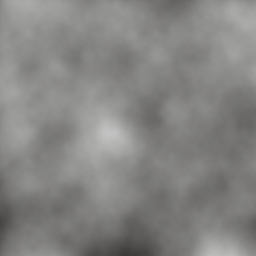
\includegraphics[width=0.25\textwidth]{figure/heightmap.png}
  \caption{An example heightmap generated using Perlin Noise}
  \label{fig:heightmap}
\end{figure}

We plan to generate the heightmap using multiple layers of simplex noise.
Simplex noise is a type of gradient noise commonly used in computer graphics and procedural generation.
The so-called gradient noise is where a psuedo-random gradient(or slope) is generated at regularly spaced points in space.
The points are then interpolated using a smoothing function to achieve a wave-like texture fitting for representing the terrain.
Each octave, or layer, of simplex noise will represent different levels of terrain granularity.
Higher frequency of noise corresponds to an area on the heightmap where we would like to generate an area with a small, yet intense difference in elevation.
Whereas lower frequencies will correspond to areas of a less intense, but larger difference in elevation forming the contour of the terrain.

The color of the terrain will be based on the height levels e.g.\ grasslands near sea level, rocky mountain textures for the taller regions, and snow for top peaks of some of the taller mountains.
One approach for achieving this is a technique called Texture splatting that is commonly used for terrain rendering.
This method consists of combining different textures blended together according to an alphamap, also referred to as a weightmap or splatmap.
Figure~\ref{fig:texture-splatting} demonstrates this technique in action.

\begin{figure}[h]
  \centering
  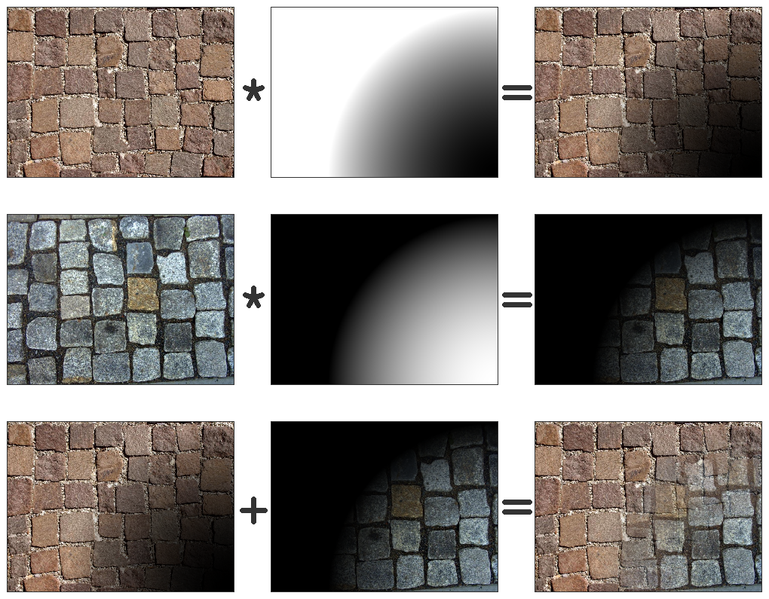
\includegraphics[width=0.4\textwidth]{figure/texture-splatting.png}
  \caption{Example of texture splatting from related work \cite{wiki:texture-splatting-img}}
  \label{fig:texture-splatting}
\end{figure}

Furthermore the user can provide a threshold height for the sea level where any point of the terrain below this threshold value will fill the valley or space with water.

If there is still time after previously mentioned implementations we intend to make the terrain more interesting by generating trees and grass throughout the world.
The way we intend to do this is to use poisson disc sampling to distribute points for trees in a natural looking fashion. % source: https://odr.chalmers.se/handle/20.500.12380/244588


\subsubsection{PopulationGenerator}
\subsection{Road}
\begin{center}
  \textit{Terrain, Population map} $\rightarrow$ \textbf{RoadGenerator} $\rightarrow$ \textit{Road network} 
\end{center}
Road generation is what will design the entire city, and it will do it by placing different kinds of roads.
We will approach this generation by first allowing the user to decide where city generation shall commence by giving them the option to place a population markers for the roads to be constructed.
The size of the city generated is defined by the user, maximum being the size of the available landscape.
Cities far away from each other will be connected by highways, and there can exist a randomly generated 

\subsubsection{Plotting out cities}
The user should be able to specify exactly where cities should begin their generation sequence.
They will do this via population markers.
Each city has a type which describes the general appearance and layout of the city.
Some examples of city type generation strategies are;
\begin{itemize}
  \item Paris strategy, which would generate circular cities with roads extending from the middle and outwards.
  \item Manhattan strategy, which consists of lots of straight roads going through the city perpendicular to other roads, creating a grid-like appearance.
  \item Chaotic strategy, completely random with lots of turning, no structure whatsoever.
\end{itemize}

Multiple cities can be plotted out at once, and generally when a road leaves the bounds of the city it converts to a highway which aims to connect to other denser areas.

\subsubsection{Main road generation}
Main roads, and roads in general, are generated by what is called `Agents'.
These only have one job, and that is to walk arond the landscape and leave roads behind them.
The agents generate the main roads depending on if it is inside a city, and what type of city it is.
All agents have a strategy that they will follow, instructing them how they should move around.
Agent strategies also tells the agent when it should terminate.

This type of generation results in a lot of flexibility, because each agent can be instructed to walk around differently.
For Paris strategy, some agents are configured to walk around in circles around the center point and others are configured to walk roughly straight outwards from the center.
For Manhattan strategy, the agents simply create completely straight roads, some agents are rotated by 90 degrees to create the perpendicular roads.

This also means agents can decide to switch strategy depending on some criteria, for example when an agent leaves the bounds of a city, it can change its strategy to a highway-type strategy.

Highways are a type of main road, and agents that have a strategy that creates highways should attempt to follow the population map towards higher density areas.
This helps cities to connect to eachother, because highways generally do not turn around as much as other main roads and it will eventually find a higher density area in the population map to go towards.

However, higher density areas does not mean there is always a city located there, it might find an area without a city.
The idea is that the highway strategy can also create new cities or villages if it comes across a very dense area and has not connected to an existing city.
There are cases where a city can be created right next to another city, but that would just result in both cities merging into one.

\subsubsection{Street generation}
While generating main roads, new agents are created which branch off the main road to create streets.
These are generally straight and grid-like, to mimic the patterns found in most neighborhoods.
However, different kind of street strategies can be created to mimic other types of neighborhoods.
To ensure that streets do not cut off main roads, these agents are given a lower priority which ensures that they are always created after main roads are finished generating.
The agents are then prioritized according to the order they were created, which means an agent will generate an entire neighborhood before the next street agent begins.
This creates clearer patterns around the city with less agents competing over the same area.

Agents with a street strategy will always look up the population map before placing a road or branching.
Higher density means a higher chance of branching, creating denser neighborhoods near the center of the city.
An agent that tries to travel into a place with too little of a population density will simply terminate without creating a road. 

\subsection{Block}
\begin{center}
    \textit{Road network, Population map} $\rightarrow$ \textbf{BlockGenerator} $\rightarrow$ \textit{Block{[}{]}}
\end{center}
This generator will from the roads and streets, and the population map, generate all the blocks used in the world.
Formal definition of Block:
\begin{center}
    \textit{Finite area connected to 1 or more streets that contains 1 or more plots.}
\end{center}
An example of this can be found in figure \ref{fig:generatorexamples}, in picture 3, the inner roads of the center area is the streets that connect and is the base for the three blocks.
After all the roads has been generated, doing most of the work structuring the world, blocks can be mapped upon the world to give it life.
Via the \textit{Road network} and \textit{Population map}, different blocks can be created. 
The main technique that will be used to find the blocks created out of the \textit{Road network} is something called Minimum Cycle Basis.
It's an algorithm used to find all cycles, which we will call blocks, withing a undirected graph, which will be all the roads and streets. 
The population map will have an effect when specifing the blocks. 
\subsection{Plot Generator}
\begin{center}
    \textit{Block, Population map} $\rightarrow$ \textbf{PlotGenerator} $\rightarrow$ \textit{Plot{[}{]}}
\end{center}
This generator will divide a \textit{Block} into multiple plots of land where buildings and parks can be built.
These \textit{Plots} are formally defined in the glossary.
Plots can not be divided into smaller pieces, they should be seen as the smallest polygon area where buildings and parks can be built.

An example of plot generation can be found in Figure~\ref{fig:generatorexamples3}.
The areas separated by the blue lines represent the \textit{Plots}.
These can be generated quite arbitrarily, and do not need to be of similar sizes.
In this case they could all represent different buildings, but parks are also valid candidates.
The only requirement is that they need to have enough room for something to be built.
One suggestion is to investigate using Voronoi diagrams for generating the \textit{Plots}, both with Euclidean distance and with Manhattan distance.

The population map can be used to determine what kind of building type is most suitable.
For instance a villa would fit well if the plot should cover a small population, while a skyscraper or an apartment complex would be suitable for high population.

\subsection{Building}
\begin{center}    
    \textit{Plot} $\rightarrow$ \textbf{BuildingGenerator}
\end{center}
This building generator will generate a single building upon a given \textit{Plot}. 
The size of the \textit{Plot} as well as the required population will be an important factor for the generation and placement of the building. 
The plan is to implement stochastic bracketed L-systems for the generation of these buildings.

\subsection{ParkGenerator}
\begin{center}
    \textit{Plot} $\rightarrow$ \textbf{ParkGenerator}                        
\end{center}
This park generator will generate a park in a given \textit{Plot}. 
The generator will try to place a few paths inside the plots. 
This to simulate a normal park where people can take walks or go for a run.
Objects such as trees, small sheds, park benches, and garbage cans will also be generated within the parks.
